\subsubsection{Ottavo periodo (2024/03/25 - 2024/04/07)}
\subsubsubsection{Planning}
\subsubsubsubsection*{Attività pianificate}
All'inizio del periodo ad ogni membro del gruppo sono stati assegnati ruoli specifici, di seguito riportati:
\begin{table}[H]
\centering
\begin{tabular}{|c|c|c|}
\hline
\textbf{Membro} & \textbf{Ruolo} \\
\hline
Samuele V. & Programmatore \\
\hline
Michele Z. & Amministratore \\
\hline
Leonardo B. & Programmatore \\
\hline
Riccardo Z. & Responsabile \\
\hline
Filippo T. & Programmatore \\
\hline
Davide B. & Responsabile \\
\hline
\end{tabular}
\caption{Ruoli assunti per ciascun membro del team all'inizio del periodo}
\end{table}
Gli obiettivi posti per lo $\textit{sprint}_G$ sono stati i seguenti:
\begin{itemize}
    \item Per quanto riguarda il \emph{PoC}:
    \begin{itemize}
        \item Raggiungere una prima implementazione della schermata di login (lato front-end);
        \item Raggiungere una prima implementazione della funzionalità di $\textit{prenotazione}_G$ (lato back-end e front-end);
        \item Raggiungere una prima implementazione della funzionalità di $\textit{ordinazione}_G$ (lato back-end e front-end) esplorando i \emph{socket} per la comunicazione bidirezionale.
    \end{itemize}
    \item Aggiornare il documento \emph{Norme di Progetto} apportando le seguenti modifiche:
    \begin{itemize}
        \item Specificare in modo maggiormente dettagliato i ruoli;
        \item Aggiungere le nuove $\textit{repository}_G$ create e la loro organizzazione;
        \item Aggiungere tra i $\textit{processi di supporto}_G$ le attività di verifica e di gestione della qualità;
        \item Specificare l'utilizzo delle nuove automazioni aggiunte recentemente.
    \end{itemize}
    \item Redigere una prima versione del glossario;
    \item Redigere una prima versione della sezione \emph{Qualità di Prodotto} e di \emph{Test di Sistema} nel documento \emph{Piano di Qualifica};
    \item Aggiornare i periodi precedenti nel \emph{Piano di Progetto} andando a definire un modo sistematico per calcolare le ore preventivate ed effettive;
    \item Rivedere i costi e le scadenze in fase di $\textit{candidatura}_G$.
\end{itemize}
\subsubsubsubsection*{Preventivo}
\begin{table}[H]
    \centering
\begin{spreadtab}{{tabular}{|c|c|c|c|c|c|c|c|}}
    \hline
    @\textbf{Membro} & @\textbf{Re} & @\textbf{Amm} & @\textbf{An} & @\textbf{Progr} & @\textbf{Proge} & @\textbf{Ve} & @\textbf{Totale} \\
    \hline
    @ Samuele V.   & 0          & 0          & 0        & 5          & 0     & 0     & sum(b2:g2) \\
    @ Leonardo B.  & 0         & 0          & 0        & 5        & 0     & 0    & sum(b3:g3) \\
    @ Riccardo Z.  & 4.5          & 0          & 0          & 0.17          & 0     & 1.5  & sum(b4:g4) \\
    @ Davide B.    & 4          & 0         & 0      & 0       & 0     & 0     & sum(b5:g5) \\
    @ Michele Z.   & 0          & 4          & 0         & 0          & 0     & 0.17     & sum(b6:g6) \\
    @ Filippo T.   & 0          & 0          & 0         & 5          & 0     & 0     & sum(b7:g7) \\
    \hline
    @\textbf{Ore totali} & sum(b2:b7) & sum(c2:c7) & sum(d2:d7) & sum(e2:e7) & sum(f2:f7) & sum(g2:g7) &  sum(b8:g8)\\
    \hline
    @\textbf{Costo totale} & 30*b8 & 20*c8 & 25*d8 & 15*e8 & 25*f8 & 15*g8 & sum(b9:g9)\\
    \hline
\end{spreadtab}
    \caption{Preventivo orario ed economico parziale per l'ottavo periodo, in base al ruolo}
    \label{tab:prev_rtb}
    \vspace{5mm}
    \textbf{Legenda:} \textit{Re} = Responsabile, \textit{Amm} = Amministratore, \textit{An} = Analista, \textit{Progr} = Programmatore, \textit{Proge} = Progettista, \textit{Ve} = Verificatore
\end{table}

\begin{figure}[H]
  \centering
  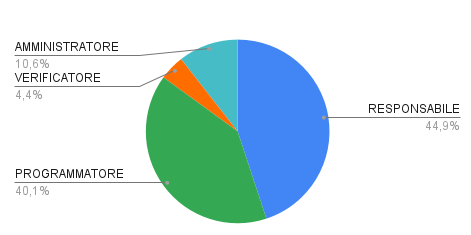
\includegraphics[width=0.6\linewidth]{grafici/8_periodo_torta.png}
  \caption{Ripartizione dei costi per ruolo nel $8^\circ$ periodo}
        \vspace{5mm}
  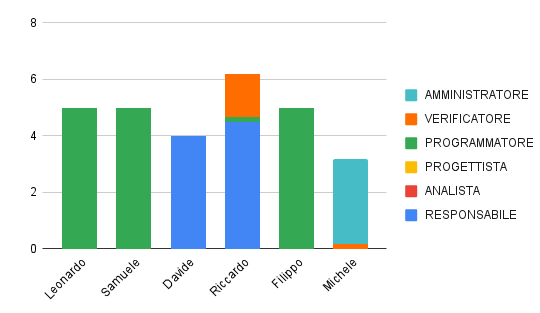
\includegraphics[width=0.7\linewidth]{grafici/8_periodo_istogramma.png}
  \caption{Ore preventivate per ciascuna persona nel $8^\circ$ periodo}
\end{figure}

\subsubsubsection{Review}
\subsubsubsubsection*{Attività svolte}
Le attività svolte in questo periodo sono state le seguenti:
\begin{itemize}
    \item Redatta ed approvata una prima versione del glossario tecnico;
    \item Redatte le sezioni \emph{Qualità di Prodotto} e \emph{Test di sistema} nel documento \emph{Piano di Qualifica};
    \item Aggiornato \emph{Norme di Progetto} con le attività di verifica, gestione della qualità e la procedura per la redazione del glossario;
    \item Rivisti i costi stabiliti in fase di $\textit{candidatura}_G$;
    \item Integrati i $\textit{websocket}_G$ nel $\textit{PoC}_G$, implementate le funzionalità di $\textit{prenotazione}_G$ e $\textit{ordinazione}_G$, non quella di login e raggiunta una configurazione soddisfacente;
    \item Richiesto un incontro con il prof. Cardin per la prima parte della revisione $\textit{RTB}_G$;
    \item Richiesto e fissato un incontro con il proponente in data 11 aprile per presentare il $\textit{PoC}_G$.
\end{itemize}
\subsubsubsubsection*{Consuntivo}
\begin{table}[H]
    \centering
\begin{spreadtab}{{tabular}{|c|c|c|c|c|c|c|c|}}
    \hline
    @\textbf{Membro} & @\textbf{Re} & @\textbf{Amm} & @\textbf{An} & @\textbf{Progr} & @\textbf{Proge} & @\textbf{Ve} & @\textbf{Totale} \\
    \hline
    @ Samuele V.   & 0          & 0          & 0         & 6          & 0     & 0     & sum(b2:g2) \\
    @ Leonardo B.  & 0         & 0          & 0        & 5.42        & 0     & 0    & sum(b3:g3) \\
    @ Riccardo Z.  & 6.75          & 0          & 0          & 0.17         & 0     & 2   & sum(b4:g4) \\
    @ Davide B.    & 5          & 0         & 0       & 0       & 0     & 0     & sum(b5:g5) \\
    @ Michele Z.   & 0          & 4.25          & 0         & 0          & 0     & 0.17     & sum(b6:g6) \\
    @ Filippo T.   & 0          & 0          & 0         & 8.5          & 0     & 0     & sum(b7:g7) \\
    \hline
    @\textbf{Ore totali} & sum(b2:b7) & sum(c2:c7) & sum(d2:d7) & sum(e2:e7) & sum(f2:f7) & sum(g2:g7) &  sum(b8:g8)\\
    \hline
    @\textbf{Costo totale} & 30*b8 & 20*c8 & 25*d8 & 15*e8 & 25*f8 & 15*g8 & sum(b9:g9)\\
    \hline
\end{spreadtab}
    \caption{Consuntivo orario ed economico parziale per l'ottavo periodo, in base al ruolo}
    \label{tab:prev_rtb}
    \vspace{5mm}
    \textbf{Legenda:} \textit{Re} = Responsabile, \textit{Amm} = Amministratore, \textit{An} = Analista, \textit{Progr} = Programmatore, \textit{Proge} = Progettista, \textit{Ve} = Verificatore
\end{table}
\subsubsubsection{Retrospective}
Dal presente periodo sono emersi i seguenti elementi:
\begin{itemize}
    \item E' stato riscontrato durante un meeting un errore sull'automazione per i $\textit{riferimenti}_G$ del glossario, si è dunque deciso di intervenire assegnando la task apposita ad uno dei membri del gruppo dunque ricorrendo ad un innalzamento dei costi. Per mitigare tale problema si è dovuta stabilire una procedura di inserimento delle parole del glossario nei documenti e verifica dei documenti da inserire nei prossimi periodi.
    \item La finalizzazione del documento \emph{Analisi dei Requisiti} si è rivelata più difficoltosa del previsto, portando ad un innalzamento dei costi e facendo emergere delle attività di verifica lacunose e da rivedere per le prossime stesure dei documenti. Per mitigare tale problema si è stabilito che debbano esistere delle procedure da seguire per poter segnare come "verificato" un documento, in particolare si aggiorneranno nei prossimi periodi le sezioni relative a ciascun documento.
\end{itemize}


%\subsubsubsubsection*{Rischi verificati}
%\subsubsubsubsection*{Analisi retrospettiva}